% !TeX root = Bericht.tex
% !TeX spellcheck = de_DE
\section{Ergebnisse}

In diesem Kapitel werden die Resultate der Messungen präsentiert, sowie die für die Versuche gewählten Einstellungen spezifiziert. 
\setcounter{subsection}{-1}

\subsection{Aufgabe 0: Bandlücke}
\textit{Diskutieren Sie warum (welche) Elektronen die Hürde von $1.115 \unit{eV}$ überwinden
	können, wo doch die mittlere Energie der Elektronen durch die thermische Bewegung nur
	$E_\mathrm{kin} = 3/2 k_B T$ ist.}


Wie bereits angedeutet, handelt es sich bei dem angegebenen $E_\mathrm{kin}$ um eine gemittelte kinetische Energie. Somit gibt es auch Teilchen mit Energiewerten, die deutlich größer sind und somit die Bandlücke überspringen können. Dabei handelt es sich um die Elektronen im Valenzband, welche also am nächsten zum Leitungsband liegen. 

%\begin{figure}[H]
%    \centering
%    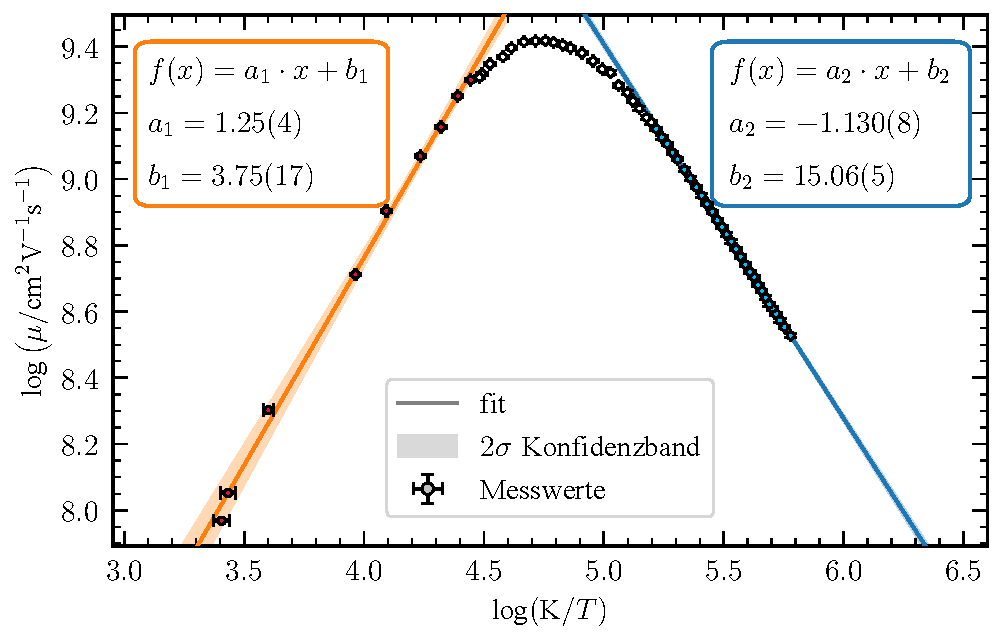
\includegraphics[width=\textwidth]{plot3.pdf}
%    \caption{}
%    \label{fig:plot3}
%\end{figure}


\subsection{Aufgabe 1: Staubkörner}

Bei den Aufnahmen des CCD-Sensors können sechseckige Staubkörner entdeckt werden. Die sechseckige Form resultiert aus der sechseckigen Geometrie des Verschlusses der Kamera. Die Staubkörner schirmen Licht nicht vollständig ab, was ein Ergebnis von Lichtbeugung an den Staubkörnern ist. 

\subsection{Aufgabe 2: Bias-Frames}
\label{subsec:ex2}
Nachdem die Temperatur des Sensors auf \SI{-20}{\degreeCelsius} abgekühlt wurde, werden 23 Bias-Frames aufgenommen, davon werden die ersten drei jedoch nicht verwendet, da diese bei diesem CCD unzuverlässige Ergebnisse liefern. Für die Auswertung werden hier die äußersten 50 Pixel auf allen Seiten der Frames ignoriert. Es ergibt sich ein mittlerer Bias von $$b^{\mathrm{ADU}}_{0}=\SI{543.40}{ADU}, $$
mit einer Standardabweichung von $$\sigma_{\mathrm{ron, 0}}^{\mathrm{ADU}}=\SI{1.81}{ADU}. $$
Ziehen wir diesen Mittelwert von einer Bias-Aufnahme ab, bleibt nur mehr das Ausleserauschen übrig. Nach diesem Abziehen ergibt sich
$$b^{\mathrm{ADU}}_{1}=\SI{0.02}{ADU}, $$
mit einem Ausleserauschen von $$\sigma_{\mathrm{ron, 1}}^{\mathrm{ADU}}=\SI{5.95}{ADU}. $$
An $b^{\mathrm{ADU}}_{1}$ sieht man, dass es fast vollständig gelingt, hier den konstanten Offset zu entfernen. 

\subsection{Aufgabe 3: Bestimmen des Gain-Faktors $g$ anhand von $\sigma_{\mathrm{ADU}}^{\mathrm{(stat)}}$ und $N_{\mathrm{ADU}}$}
Für die folgenden Messungen wurde die Blende für die blaue Folie auf \SI{16}{mm} bei einer Versorgungsspannung der Flatfield-lampe von \SI{9}{V}. Für die grüne Folie wurde die Blende auf \SI{22}{mm} und die Spannung auf \SI{8.1}{V} eingestellt. Es wurden für beide Folien (grün und blau) je eine Flatfield-Aufnahme mit Belichtungszeit von \SI{1}{s} sowie je drei Bias-Aufnahmen genommen. Verwenden wir die zwei Relationen $N^\mathrm{e}=g\cdot N^{\mathrm{ADU}}$ sowie $\sigma^\mathrm{e}=g\cdot\sigma^\mathrm{ADU}$ und die Tatsache, dass laut Poissonstatistik $\sqrt{N^e} = \sigma^e$ gilt, erhalten wir 
$$g=\frac{N^{\mathrm{ADU}}}{\sigma^{\mathrm{ADU}^2}}. $$
Der Gain-Faktor $g$ beschreibt hierbei die Umwandlung von Elektronen in Analog-Digital-Units. Die Signalstärke wird durch $N$, die Standardabweichung durch $\sigma$ symbolisiert, wobei das tiefgestellte ADU immer für das Signal in Analog-Digital-Units steht, und das tiefgestellte $e$ für die Stärke des elektronischen Signals. 
Für die grüne Folie ergab sich ein mittlerer Wert von \SI{6415.12}{ADU} mit einer Standardabweichung von \SI{55.03}{ADU}, daraus resultiert ein Gain Faktor
$$g_\text{grün}=2.11.$$ 
Analog ergibt sich für die blaue Folie ein Mittelwert von \SI{2553.77}{ADU} mit Standardabweichung \SI{35.36}{ADU}. Hier ergibt sich
$$g_\mathrm{blau}=2.04.$$ In \autoref{blau_aufgabe3} sieht man exemplarisch für die blaue Folie das Gesamtbild des CCD, sowie das ausgewählte $200\times200$ Pixel Quadrat. Es wurde eine divergierende Farbpalette gewählt, um die Inhomogenität der im Idealfall perfekten Folie hervorzuheben. Für dieses Quadrat ist darunter das Histogramm der Pixel-Sättigung sowie die Aufnahme im Detail zu sehen. Der Ausschnitt aus dem Gesamtbild weist aber eine annähernd homogene Beleuchtung auf, wie man an der Gaußähnlichen Form des Histogramms erkennen kann. Im Anhang ist die selbe Grafik auch für die grüne Folie zu sehen. 
\begin{figure}[H]
	\centering
	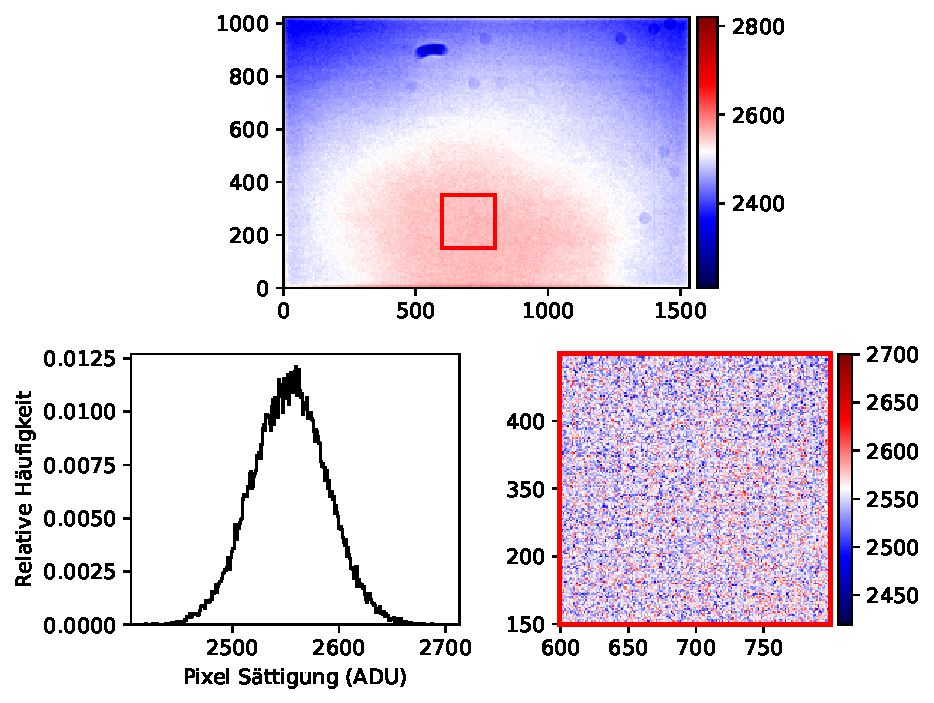
\includegraphics[width=\linewidth]{ex2_Blue}
	\caption{Zu sehen ist oben das gesamte Flatfield-Frame des CCD für die blaue Folie, rechts unten ist auf das rote Quadrat gezoomt. Das Quadrat hat eine Seitenlänge von 200 Pixeln und seine rechte untere Ecke liegt auf der x-Achse bei 600, auf der y-Achse bei 150. Links unten ist ein Histogramm der  Pixel Sättigung gezeigt.}
	\label{blau_aufgabe3}
\end{figure}





%Mean of bias: 543.3951320934171
%Standard deviation of bias: 1.8105097572355755
%Mean of data: 0.017651733711970482
%Standard deviation of data: 5.948178109814652
%danach 4,5,6, 8
\subsection{Aufgabe 4: Betrachtung des linearen Verhaltens in Abhängigkeit der Belichtungszeit}
%\begin{figure}[H]
%   \centering
%  \includegraphics{CCD/bilder/ex4.pdf}
% \caption{Zu sehen sind für beide Folien die Linearität in bezug auf die Belichtungszeit. Dabei haben wir bei dem }
%\label{fig:ex4}
%\end{figure}
Um das Verhalten in Abhängigkeit der Belichtungszeit zu untersuchen, wurden bei der blauen und grünen Folie Belichtungszeiten zwischen  $0.5 \unit{s}$ und $30 \unit{s}$ betrachtet. Für geringe sowie sehr hohe Belichtungszeiten, bei denen Sättigung auftritt, wird kein lineares Verhalten erwartet. Daher ist in diesen Bereichen die Schrittweite geringer gewählt worden. In \autoref{fig:ex4} ist für beide Farbuntersuchungen der Wert $N^\mathrm{ADU}/t_\mathrm{exp}$ gegen die Belichtungszeit $t_\mathrm{exp}$ aufgetragen, wobei die y-Achse mit dem Mittelwert, $N_\mathrm{mean}^\mathrm{ADU}$ aus dem linearen Bereich normiert wurde. Somit ist für den linearen Bereich  konstant 1 zu erwarten. im Sättigungsfall haben wir dann eine negative Steigung und im Bereich der sehr kurzen Belichtungszeit haben wir eine Steigung größer als 1. Für diese Messungen wurde dasselbe Quadrat wie bereits in \autoref{blau_aufgabe3} verwendet. \\

Woher rührt nun die Nichtlinearität bei sehr kleinen Belichtungszeiten? Nachdem die CCD durch einen mechanischen Verschluss von der Linse getrennt ist, der je nach Belichtungszeit länger oder kürzer geöffnet ist, und dieser Shutter nicht perfekt arbeitet, ist dieser Effekt gerade bei kurzen Belichtungszeiten stärker zu erkennen. Es ist zu bedenken, dass die Kappe ja eine Wegstrecke zurücklegen muss um zu Öffnen oder zu Schließen, somit gibt es einen bestimmten Zeitraum in dem eine teilweise Belichtung des CCD vorliegt. Dies lässt sich auch nicht unterdrücken. Weiters ist nicht klar, wie genau die Belichtungszeit mit dem Shutter funktioniert, also ob am Ende der Belichtungszeit der Verschluss gänzlich geschlossen sein muss, oder ob der Verschluss sein Verschließen gerade beginnt. Alle Szenarien dazwischen sind natürlich auch möglich.

\begin{figure}[H]
	\centering
	\includegraphics{ex4}
	\caption{Zu sehen ist der aufgetragene Differenzenquotient gegenüber der Belichtungszeit, wobei dabei für eine lineare Funktion, welche normiert ist, der Wert 1 angenommen wird. In nichtlinearen Bereichen ist eine Abweichung davon ersichtlich. }
	\label{fig:ex4}
\end{figure}
Der Dunkelstrom darf in dieser Untersuchung ignoriert werden, da er mit er mit dem exponentiellen Verhalten bezüglich der Temperatur, mit einem Faktor von  $\sim e^{-11.5} $ multipliziert wird (vgl. \autoref{Aufgabe8}, \autoref{temperaturplot}). Damit wird dieser vernachlässigbar klein.




\subsection{Aufgabe 5: Exaktere Bestimmung des Gains }
\label{subsec:ex5}

In \autoref{plot_aufgabe5} sehen wir das gemessene Totalrauschen in Abhängigkeit des Signals. An die Datenpunkte wurde eine Parabel angepasst, aus der sich der Gain-Faktor ergibt. Wir erhalten
$$g_\mathrm{gruen, 1} = 2.11(4) \quad \mathrm{und}\quad g_\mathrm{blau, 1} = 2.15(5).  $$
Setzt man nun den Offset der Parabel auf das in Aufgabe 2 bestimmte Ausleserauschen $\sigma_{\mathrm{ron, 1}}^{\mathrm{ADU}}$ (also der Form $f(x) = ax^2+bx + \sigma_{\mathrm{ron, 1}}^{\mathrm{ADU}}$) und passt diese erneut an die Daten an, erhalten wir fast identische Fits, die Plots hierzu sind in \autoref{fig:ex5_2} im Anhang zu finden. Dabei kommt man auf 
$$g_\mathrm{gruen, 1} = 2.13(2) \quad \mathrm{und}\quad g_\mathrm{blau, 1} = 2.16(2).  $$ und somit sind diese Werte im Rahmen der Unsicherheit vereinbar.


\begin{figure}[H]
	\centering
	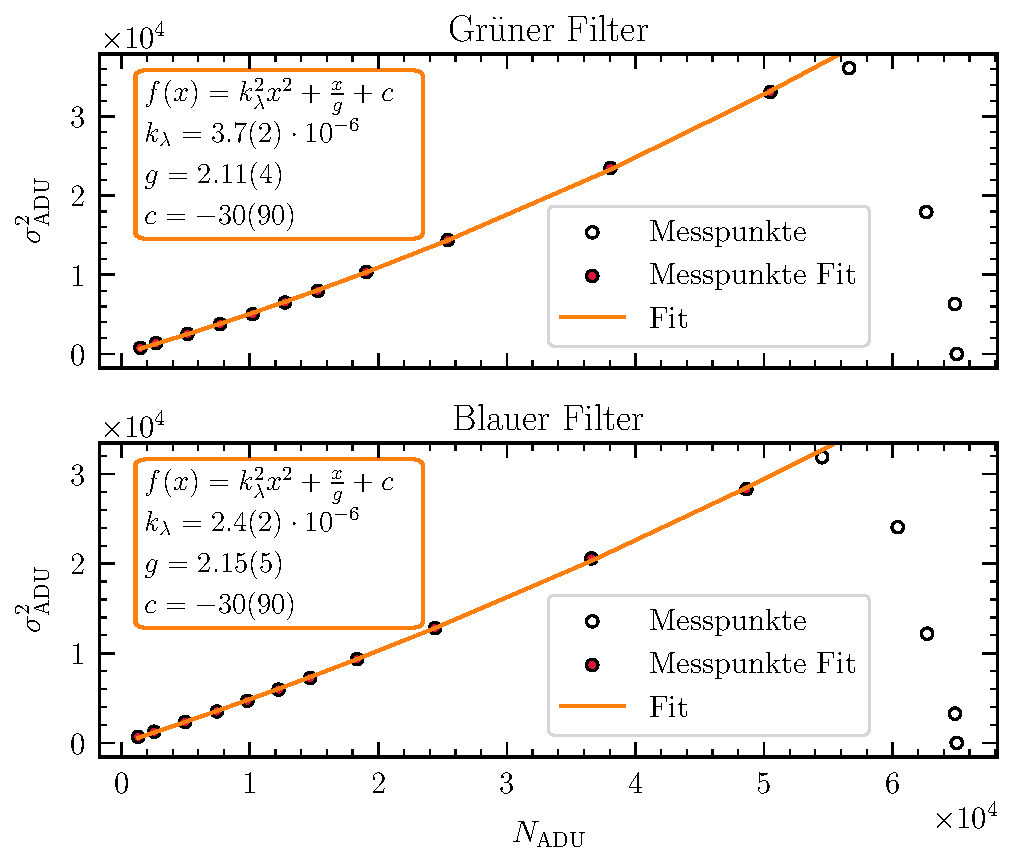
\includegraphics{ex5}
	\caption{Zu sehen ist die quadrierte Standardabweichung in ADU abhängig der Signalstärke in ADU für die grüne und die blaue Folie. Ebenso sind Fitfunktionen an die Daten angepasst worden. }
	\label{plot_aufgabe5}
\end{figure}

Eine spanndende Betrachtung hierbei ist die \textit{full well capacity}. Hierbei handelt es sich um die maximale Elektronenzahl, die in einem Potentialtopf gespeichert werden kann,  also der Punkt an dem man Sättigung erreicht und die Messwerte in \autoref{plot_aufgabe5} das zu erwartende Verhalten verlassen. Dieser ist ungefähr bei $N_\mathrm{ADU}=5.0(2) \cdot 10^4$ (Der letzte Verwendete Punkt für den Fit), was  unter Berücksichtigung des $g_\mathrm{gruen, 1} = 2.11(4) $ zu $N_\mathrm{SAT}=10.5(5) \cdot 10^4$ Elektronen. Wenn man das mit dem zugehörigen Wert aus dem Datenblatt von $N_\mathrm{SAT,Data}=10^4$ (vgl. \autocite{DATENBLATTCCD}) lässt sich eine Übereinstimmung erkennen. Da es sich hierbei nur um eine qualitative Einschätzung der Größenordnung handelt, wurde die Berechnung nur für den Grünen Filter und den Gain mittels der Bestimmung über das vorgegebene $\langle bias\rangle$ gemacht. 

Um das $\langle bias \rangle$ zu bestimmen ohne es zuvor in einer Bias-Frame Serie zu messen kann der Schnittpunkt der gefitteten Funktion mit der y-Achse herangezogen werden. Worin liegt nun der Nachteil dieser Methodik? Es ist schlicht eine Unbekannte mehr, die zu bestimmen ist, und diese könnte ein schlechteres Ergebnis für den Gainfaktor bringen. In unseren Messungen hat das jedoch keinen signifikanten Unterschied ergeben.


\subsection{Aufgabe 6: Bestimmung des Ausleserauschens in Elektroneneinheiten}
Um das Ausleserauschen des CCD-Sensors von der arbiträren Einheit $\oldunit{ADU}$ in die tatsächliche Anzahl an geflossenen Elektronen zu konvertieren müssen wir $\sigma_{\mathrm{ron, 1}}^{\mathrm{ADU}}$ mit dem Gain multiplizieren. Dafür verwenden wir für das Ausleserauschen den in \autoref{subsec:ex2} bestimmten Wert $\sigma_{\mathrm{ron, 1}}^{\mathrm{ADU}} = 5.95$. Nachdem der Gain unabhängig von der Wellenlänge abhängen sollte, mitteln wir über die in \autoref{subsec:ex5} gefitteten Gain Werte und erhalten $\bar{g} = 2.13(3)$. Damit ergibt sich für das Ausleserauschen
\begin{equation*}
	\sigma_{\mathrm{ron}}^{\mathrm{e}} = g \cdot \sigma_{\mathrm{ron}}^{\mathrm{ADU}} = 12.66(19).
\end{equation*}
Vergleicht man diesen Wert mit der Angabe des Herstellers von 15 Elektronen \autocite{DATENBLATTCCD}, so erkennt man dass wir signifikant darunter liegen. Das ist aber nicht unüblich, da Toleranzen im Datenblatt so gewählt sind, dass sie von keinem Gerät überstiegen werden. Damit werden run-to-run Varianzen berücksichtigt. 


\subsection{Aufgabe 7: Blooming}
Das Blooming ist eine phänomenologische Erscheinung, welche dadurch entsteht, dass die einzelnen Pixel nur eine begrenzte Menge an Elektronen in ihrem Potentialtopf halten können. Sollte diese Anzahl überschritten werden, wandern die Elektronen in den benachbarten Potentialtopf. Dieser Vorgang wiederholt sich weiter. Da die CCD Pixel immer in einer bestimmten Linie ausgelesen werden, ist es baulich so vorgesehen, dass die Elektronen sich in einer bestimmten Richtung leichter fortbewegen können. Daher ist in \autoref{bloomingbild} auf der rechten Seite auch eine vertikale Linie zu sehen, welche sich nach unten hin prominenter Ausbreitet. Dies entspricht der Ausleserichtung des CCD-Sensors (vgl.\autocite{Blomming}).

\begin{figure}[H]
	\centering
	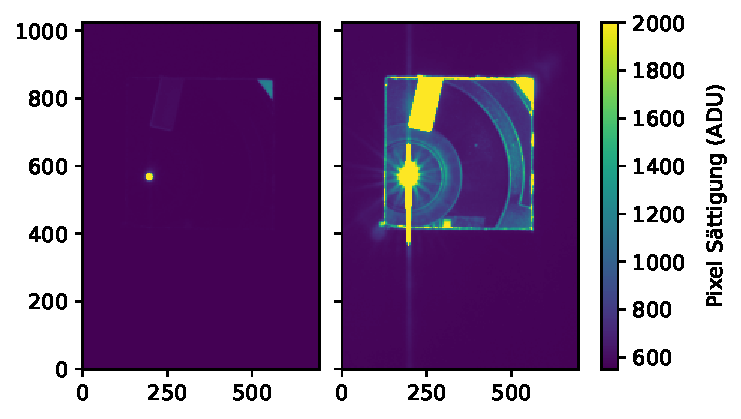
\includegraphics[width=\linewidth]{blooming}
	\caption{Zu sehen sind 2 Aufnahmen des gleichen Aufbaus mit unterschiedlicher Belichtungszeit, dabei liegt die Belichtungszeit links bei $0.1 \unit{s}$ und rechts bei $12 \unit{s}$, das Blooming ist als vertikaler Strich, welcher maximal gesättigt ist erkennbar.}
	\label{bloomingbild}
\end{figure}


\subsection{Aufgabe 8: Temperaturabhängigkeit des Dunkelstromes}
\label{Aufgabe8}
Jetzt wird die Temperaturabhängigkeit des Dunkelstromes untersucht. Dabei werden für jeden Temperaturschritt drei Darkframes und acht Bias-frames aufgenommen, von den Bias-frames werden die ersten drei wieder verworfen. Dabei wird die Temperatur in Schritten von \SI{8}{\degreeCelsius} von \SI{-20}{\degreeCelsius} bis \SI{20}{\degreeCelsius}. Die verwendete Belichtungszeit beträgt \SI{180}{s} unter \SI{-10}{\degreeCelsius}, \SI{12}{s} unter \SI{10}{\degreeCelsius} und \SI{60}{s} darüber.   
Der Dunkelstrom $I$ folgt dem Zusammenhang
\begin{equation}\label{eqn:dark}
	I= const\cdot T^{3/2}e^{-\frac{E_\mathrm{g}}{2k_\mathrm{B}T}},
\end{equation}
wobei $E_\mathrm{g}$ der Bandlücke des Materials entspricht \cite{ccd}. Als Proxy für den Dunkelstrom wurde der Mittelwert der geflossenen Elektronen hergenommen, da die genaue Umrechnungskonstante einfach in den konstanten Term in \autoref{eqn:dark} integriert werden kann. Durch Logarithmieren und Umstellen von \autoref{eqn:dark} ergibt sich ein linearer Zusammenhang, der in \autoref{temperaturplot} zu sehen ist, und für einen Fit verwendet wird. Aus zwei unterschiedlichen Regimes mit zwei unterschiedlichen Geradenfits erhalten wir zwei Werte für Bandlücken:
$$E_\mathrm{g,1}=\SI{1.1(2)}{eV} \quad\mathrm{und}\quad E_\mathrm{g,2}=\SI{-0.34}{eV}. $$ Letztere ist nicht mit einem Fehler behaftet, da eine Gerade mit zwei Freiheitsgrade an zwei Datenpunkte angepasst wurde und damit Unsicherheiten nicht sinnvoll abgeschätzt werden können.


\begin{figure}[H]
	\centering
	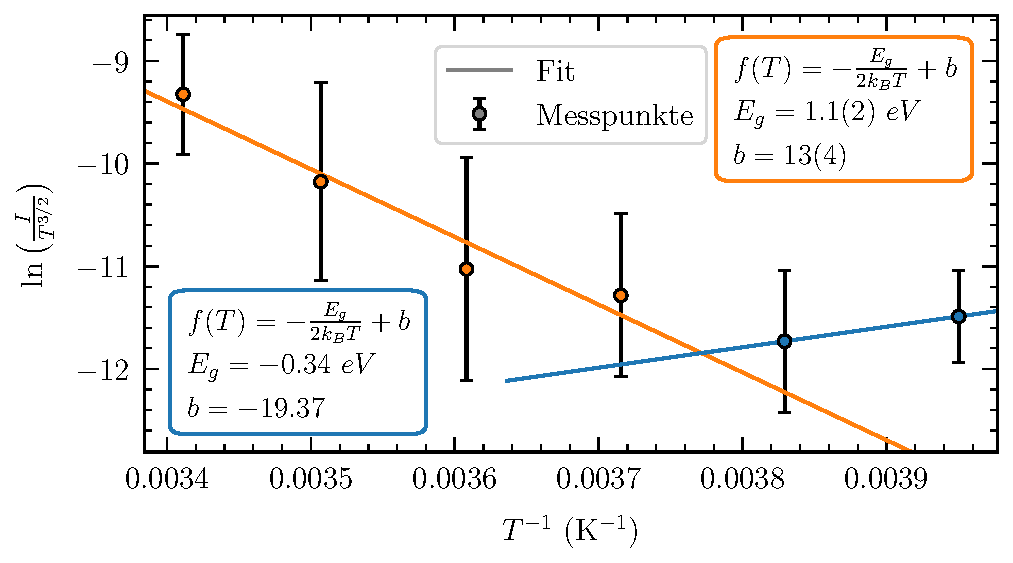
\includegraphics[width=\linewidth]{ex7}
	\caption{Zu sehen sind der Dunkelstrom (in logarithmischer Darstellung und durch $T^{3/2}$ dividiert), abhängig von der inversen Temperatur gezeigt. Für die zwei Regionen wurden zwei Fits erstellt, die Parameter des blau dargestellten weisen keine Unsicherheit auf, da sie nur durch zwei Punkte bestimmt wurden. }
	\label{temperaturplot}
\end{figure}